% Curriculum vitae
% Victor M. Fdez-Castro
% 18 January 2016

\documentclass[12pt,a4paper]{article}

\usepackage[english]{babel}
\usepackage[utf8]{inputenc}
\usepackage[table]{xcolor}
\usepackage{longtable}
\usepackage{graphicx}
\usepackage[hidelinks]{hyperref}

\title{Curriculum vitae}
\author{Víctor Manuel Fernández Castro}

\setlength{\oddsidemargin}{0pt}
\setlength{\evensidemargin}{0pt}
\setlength{\textwidth}{6in}

\newcommand{\header}[1]{\multicolumn{2}{c}{\cellcolor{black} \textcolor{white} {#1}} \\}
\renewcommand{\arraystretch}{1.5}

%-------------------------------------------------------------------------------

\begin{document}
	\large
	
	\begin{center}
		\textbf{Víctor Manuel Fernández-Castro}
	\end{center}
	
	\normalsize
	\centering

	\begin{tabular}{m{0.8\textwidth}m{0.2\textwidth}}
		2 Vire St. \newline
		Santa Fe, Granada (Spain) \newline
		January 17\textsuperscript{th}, 1990 \newline
		\newline
		+34 695 672 827 \newline
		vmfdez90@gmail.com & 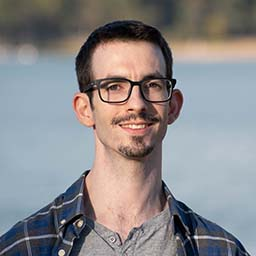
\includegraphics[width=3cm]{victor}
	\end{tabular}
	
	%---------------------------------------------------------------------------
	
	\begin{longtable}{p{0.2\textwidth}p{0.8\textwidth}}
		\\
		\header{\textbf{Education}}
		\\
		2006 -- 2008 & Bachelor of Science and Enginnering. \newline
		Jiménez de Quesada High School. Santa Fe (Granada). \\
		2008 -- present & Computer Engineering at University of Granada.
		\begin{itemize} \itemsep 0pt \parskip 0pt
			\item Cryptography.
			\item Computer graphics.
			\item Parallel computing.
			\item Algorithmics ---with outstanding---.
			\item Design of operating systems ---with outstanding---.
			\item Specialized architectures ---with outstanding and Honors---.
		\end{itemize} \\
		Mar. -- May 2015 & Workshop about information resources at academic library. \\
		2015 -- 2016 & Workshop about Sketchup and Lumion by \textit{InterCambia 
		ETSAG}. \\
		Jan. 2016 & Workshop about LaTeX and Git by \textit{Darwin Eventur}. \\
		\\
		\header{\textbf{University experience}}
		\\
		Sept. 2015 & Presentation of final project: \textit{``Remote 
		interpretation of scores on wind instruments''}, with outstanding and 
		Honors. \\
		2013 -- 2014 & Erasmus scholarship at Polytechnic University of Milan
		(Italy).
		\begin{itemize} \itemsep 0pt \parskip 0pt
			\item Design and implementation of mobile applications.
			\item Code transformation and optimization.
			\item Computer security.
		\end{itemize} \\
		\\
		\header{\textbf{Work experience}}
		\\
		2014 -- 2015 & Practices at Wap Manía S.L. as designer and programmer 
		for Android and web applications. \\	
		2011 -- present & Science, programming and piano support teacher. \\
		\\
		\header{\textbf{Skills profile}}
		\\
		Languages & Spanish (native). \newline
		English (high level). \newline
		Italian (middle level). \newline
		French (basic level). \\
		Programming & C/C++, Java, C\#, Python, PHP, HTML5/CSS, JavaScript, 
		Bash, Lisp, Prolog, LaTeX, MATLAB, Mathematica. \\
		Frameworks & POSIX, MPI, OpenMP, OpenGL, Qt, Android, Processing. \\
		Platforms & Linux, Windows, Android, Arduino, Raspberry Pi. \\
		Technologies & Web, Git, LaTeX, Doxygen. \\
		Databases & MySQL, SQLite, Oracle. \\
		Driving license & Category B (cars). \\
		\\
		\header{\textbf{Interests and activities}}
		\\
		1998 -- 2008 & Elementary Grade to 4\textsuperscript{th} of Professional
		Grade of piano at Conservatory \textit{Ángel Barrios} of Granada. \\
		2010 -- 2013 & Founded and participated as pianist in the band 
		\textit{Milestones}. \\
		2010 -- present & Solist pianist at Musical Evenings at ETSIIT (Granada). \\
		2010 -- present & Blog about computers: 
		\href{http://vikman90.blogspot.com}{vikman90.blogspot.com}. \\
		2015 -- present & GitHub account: 
		\href{https://github.com/vikman90}{vikman90}. \\
	\end{longtable}
\end{document}

